\begin{solution}
\begin{enumerate}
\item {[7 points]} Substituting the expression for $u(x,y,t)$ into the partial differential equation yields
\[
\sum_{j=1}^\infty \sum_{k=1}^\infty a_{j,k}''(t) \psi_{j,k}(x,y) = \sum_{j=1}^\infty \sum_{k=1}^\infty a_{j,k}(t) \left(-\left(L\psi_{j,k}\right)(x,y)\right)
\]
and hence
\[
\sum_{j=1}^\infty \sum_{k=1}^\infty a_{j,k}'' (t) \psi_{j,k}(x,y) = \sum_{j=1}^\infty \sum_{k=1}^\infty \left(-\lambda_{j,k}\right)a_{j,k}(t)\psi_{j,k}(x,y).
\]
We can then say that
\begin{eqnarray*}
&&\sum_{j=1}^\infty \sum_{k=1}^\infty a_{j,k}'' (t) \int_0^1\int_0^1\psi_{j,k}(x,y)\psi_{m,n} (x,y)\,dx\,dy
\\
&=&\sum_{j=1}^\infty \sum_{k=1}^\infty \left(-\lambda_{j,k}\right)a_{j,k}(t)\int_0^1\int_0^1\psi_{j,k}(x,y)\psi_{m,n} (x,y)\,dx\,dy
\end{eqnarray*}
for $m,n=1,2,\ldots$, from which it follows that
\[
a_{m,n}''(t)=-\lambda_{m,n} a_{m,n}(t),
\]
for $m,n=1,2,\ldots$, since
\[
\int_0^1\int_0^1\psi_{j,k} (x,y)\psi_{m,n} (x,y)\,dx\,dy = \left\{\begin{array}{ll} 1 & \mbox{if }j=m\mbox{ and }k=n \\ 0 & \mbox{if }j\ne m\mbox{ or }k\ne n \end{array}\right.
\]
for $j,k,m,n=1,2,\ldots$.

Also,
\[
u(x,y,0)=u_0(x,y)
\]
means that
\[
\sum_{j=1}^\infty \sum_{k=1}^\infty a_{j,k}(0) \psi_{j,k} (x,y)=u_0(x,y)
\]
and so
\[
\sum_{j=1}^\infty \sum_{k=1}^\infty a_{j,k}(0) \int_0^1\int_0^1\psi_{j,k} (x,y)\psi_{m,n} (x,y)\,dx\,dy=\int_0^1\int_0^1u_0(x,y)\psi_{m,n}(x,y)\,dx\,dy,
\]
for $m,n=1,2,\ldots$, from which it follows that
\[
a_{m,n}(0)=\int_0^1\int_0^1u_0(x,y)\psi_{m,n}(x,y)\,dx\,dy,
\]
for $m,n=1,2,\ldots$, since
\[
\int_0^1\int_0^1\psi_{j,k} (x,y)\psi_{m,n} (x,y)\,dx\,dy = \left\{\begin{array}{ll} 1 & \mbox{if }j=m\mbox{ and }k=n \\ 0 & \mbox{if }j\ne m\mbox{ or }k\ne n \end{array}\right.
\]
for $j,k,m,n=1,2,\ldots$.

Moreover,
\[
u_t(x,y,t)=\sum_{j=1}^\infty \sum_{k=1}^\infty a_{j,k}' (t) \psi_{j,k}(x,y).
\]
Hence,
\[
u_t(x,y,0)=0
\]
means that
\[
\sum_{j=1}^\infty \sum_{k=1}^\infty a_{j,k}'(0) \psi_{j,k} (x,y)=0
\]
and so
\[
\sum_{j=1}^\infty \sum_{k=1}^\infty a_{j,k}'(0) \int_0^1\int_0^1\psi_{j,k} (x,y)\psi_{m,n} (x,y)\,dx\,dy=\int_0^1\int_0^10\,dx\,dy,
\]
for $m,n=1,2,\ldots$, from which it follows that
\[
a_{m,n}'(0)=0,
\]
for $m,n=1,2,\ldots$, since
\[
\int_0^1\int_0^1\psi_{j,k} (x,y)\psi_{m,n} (x,y)\,dx\,dy = \left\{\begin{array}{ll} 1 & \mbox{if }j=m\mbox{ and }k=n \\ 0 & \mbox{if }j\ne m\mbox{ or }k\ne n \end{array}\right.
\]
for $j,k,m,n=1,2,\ldots$, and
\[
\int_0^1\int_0^10\,dx\,dy=0.
\]

Hence, for $j,k=1,2,\ldots$, $a_{j,k}(t)$ is the solution to the differential equation
\[
a_{j,k}''(t)=-\lambda_{j,k} a_{j,k}(t)
\]
with initial conditions
\[
a_{j,k}(0)=\int_0^1\int_0^1u_0(x,y)\psi_{j,k}(x,y)\,dx\,dy
\]
and
\[
a_{j,k}'(0)=0.
\]

\item {[4 points]} For $j,k=1,2,\ldots$, the differential equation $a''_{j,k}(t) = -\lambda_{j,k} a_{j,k}(t)$ has solutions of the form
\[
a_{j,k}(t) = A_{j,k}\sin\left(\sqrt{\lambda_{j,k}} t\right)+B_{j,k}\cos\left(\sqrt{\lambda_{j,k}} t\right)
\]
with the constants $A_{j,k}$ and $B_{j,k}$ being determined by the initial conditions. Evaluating the general solution at $t=0$ gives
\[
B_{j,k}=a_{j,k}(0)
\]
and so
\[
a_{j,k}(t) = A_{j,k}\sin\left(\sqrt{\lambda_{j,k}} t\right)+{100 (5+7(-1)^j)(5+7(-1)^k)\over j^3 k^3 \pi^6}\cos\left(\sqrt{\lambda_{j,k}} t\right)
\]
since
\[
a_{j,k}(0)=\int_0^1\int_0^1u_0(x,y)\psi_{j,k}(x,y)\,dx\,dy={100 (5+7(-1)^j)(5+7(-1)^k)\over j^3 k^3 \pi^6}.
\]
Computing the derivative
\[
a'_{j,k}(t) = A_{j,k}\sqrt{\lambda_{j,k}} \cos(\sqrt{\lambda_{j,k}} t) - {100 (5+7(-1)^j)(5+7(-1)^k)\over j^3 k^3 \pi^6}\sqrt{\lambda_{j,k}} \sin(\sqrt{\lambda_{j,k}} t)
\]
and evaluating it at $t=0$ then gives
\[
a'_{j,k}(0) = A_{j,k}\sqrt{\lambda_{j,k}}
\]
and so
\[
A_{j,k} = 0
\]
since
\[
a'_{j,k}(0) = 0.
\]

Therefore, for $j,k=1,2,\ldots$,
\begin{eqnarray*}
a_{j,k}(t)&=&{100 (5+7(-1)^j)(5+7(-1)^k)\over j^3 k^3 \pi^6}\cos\left(\sqrt{\lambda_{j,k}} t\right)
\\
&=&{100 (5+7(-1)^j)(5+7(-1)^k)\over j^3 k^3 \pi^6}\cos\left(\pi\sqrt{j^2+k^2} t\right).
\end{eqnarray*}
\\
\item {[4 points]} We can write
\begin{eqnarray*}
u(x,y,t) &=& \sum_{j=1}^\infty \sum_{k=1}^\infty a_{j,k}(t) \psi_{j,k}(x,y)
\\
&=& \sum_{j=1}^\infty \sum_{k=1}^\infty {100 (5+7(-1)^j)(5+7(-1)^k)\over j^3 k^3 \pi^6}\cos\left(\pi\sqrt{j^2+k^2} t\right) \psi_{j,k}(x,y)
\\
&=& \sum_{j=1}^\infty \sum_{k=1}^\infty {200 (5+7(-1)^j)(5+7(-1)^k)\over j^3 k^3 \pi^6}\cos\left(\pi\sqrt{j^2+k^2} t\right) \sin(j\pi x)\sin(k\pi y).
\end{eqnarray*}
\\
\item {[10 points]} The requested plots are below.

\begin{center}
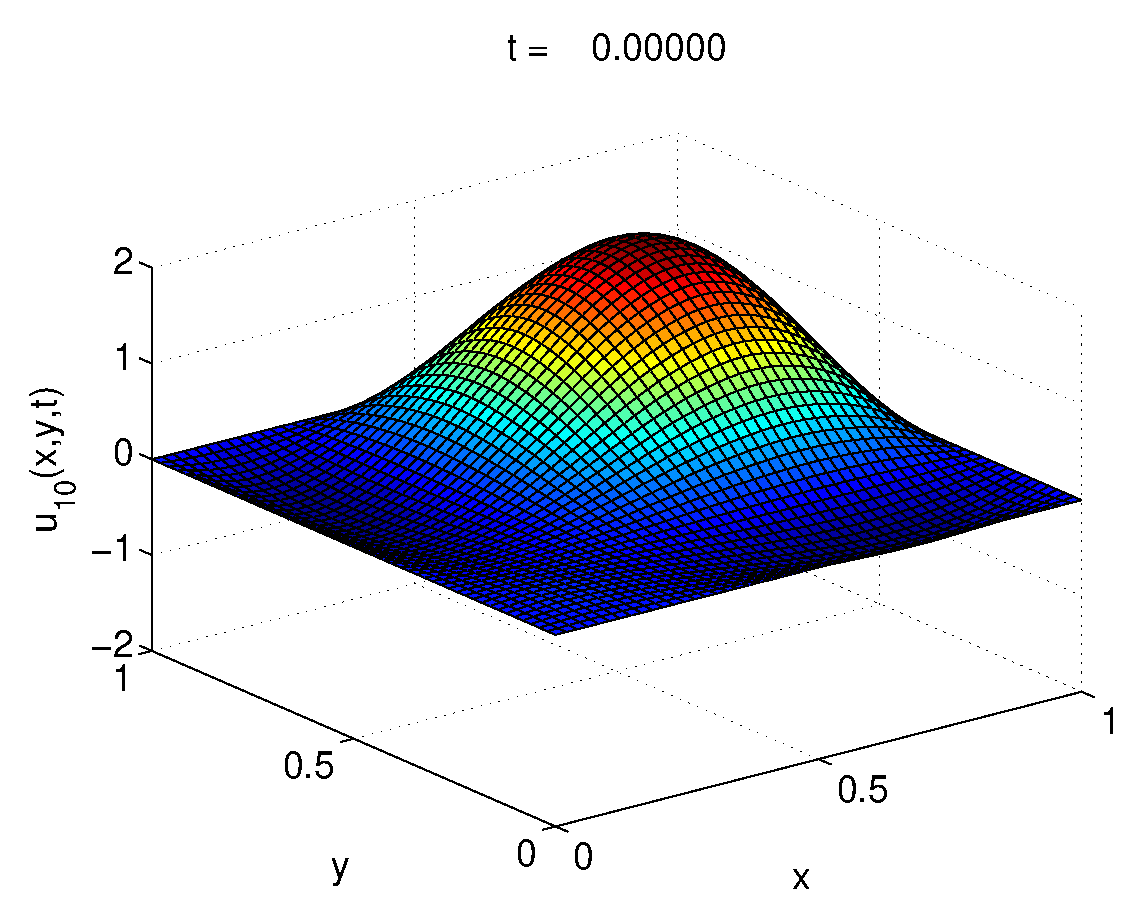
\includegraphics[scale=0.37]{wave2d_1} \quad
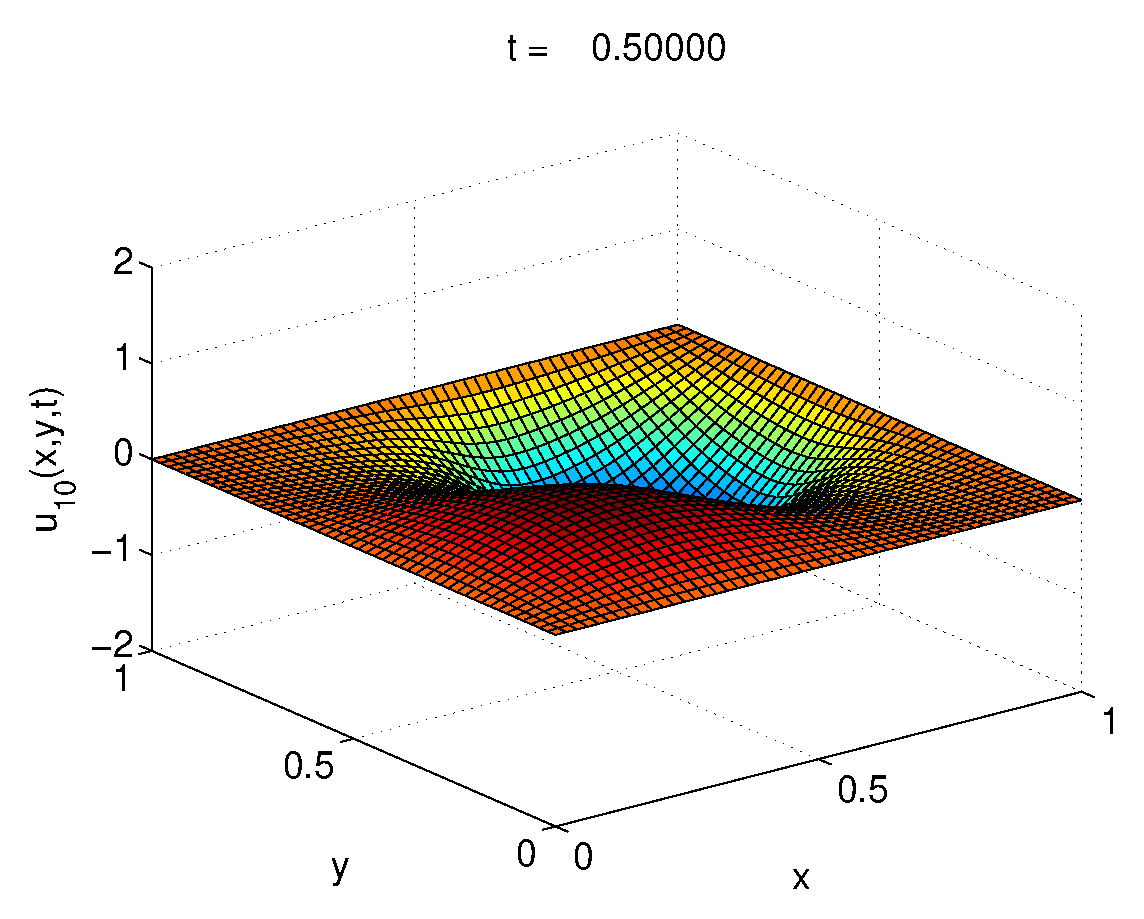
\includegraphics[scale=0.37]{wave2d_2} 

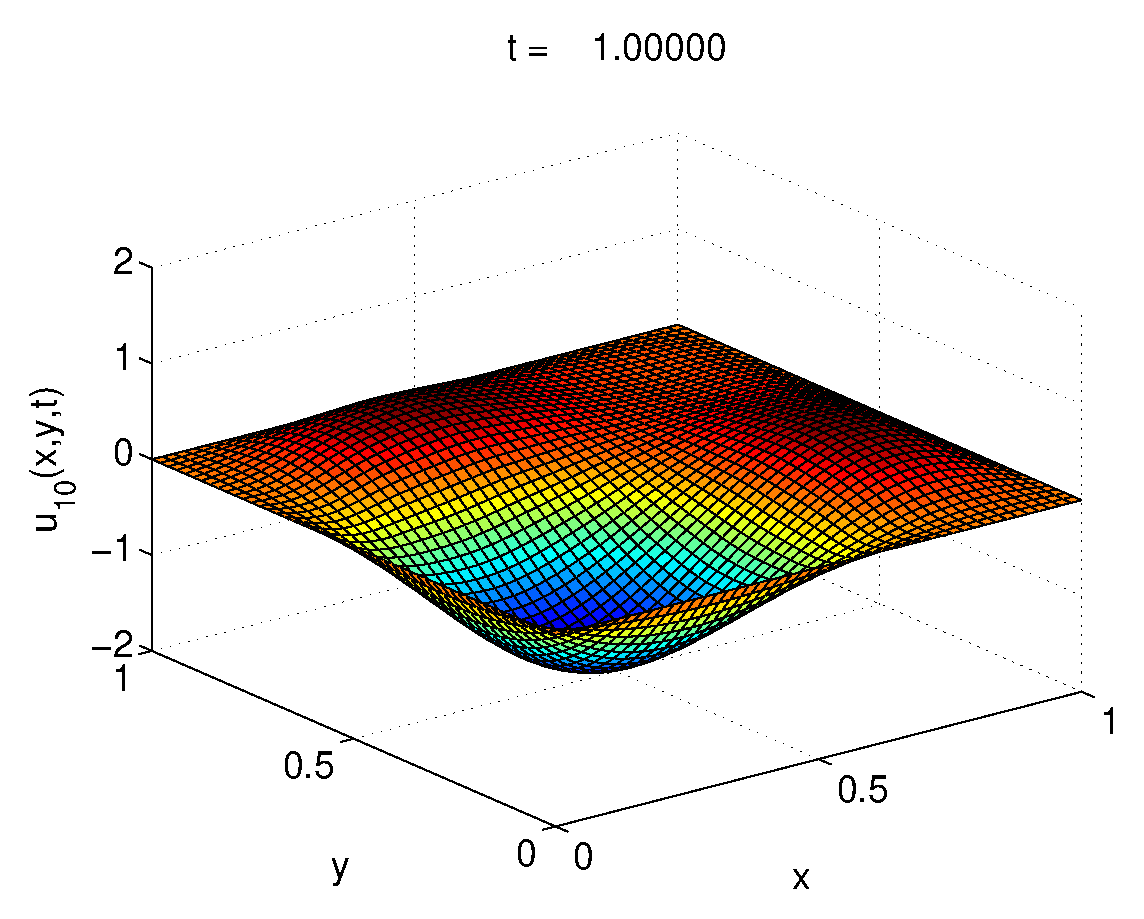
\includegraphics[scale=0.37]{wave2d_3} \quad
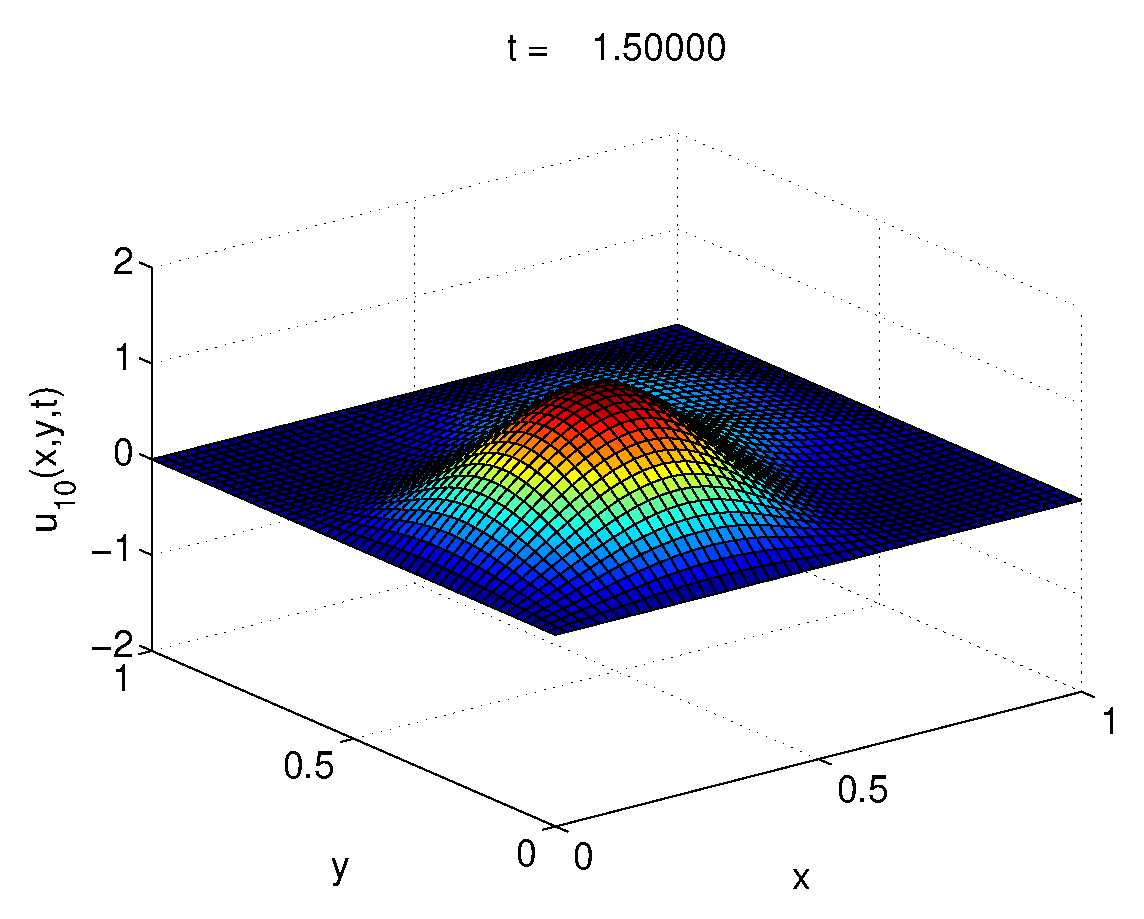
\includegraphics[scale=0.37]{wave2d_4}

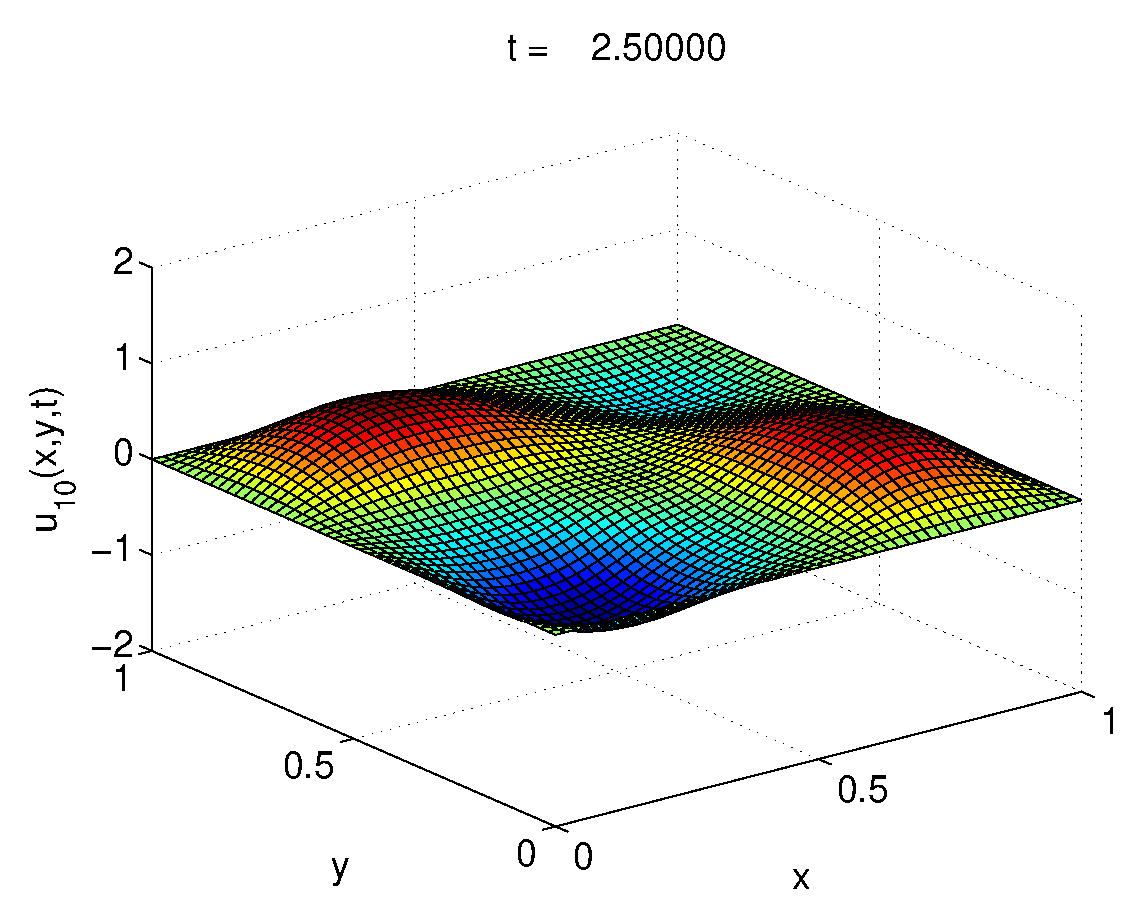
\includegraphics[scale=0.37]{wave2d_5} \quad
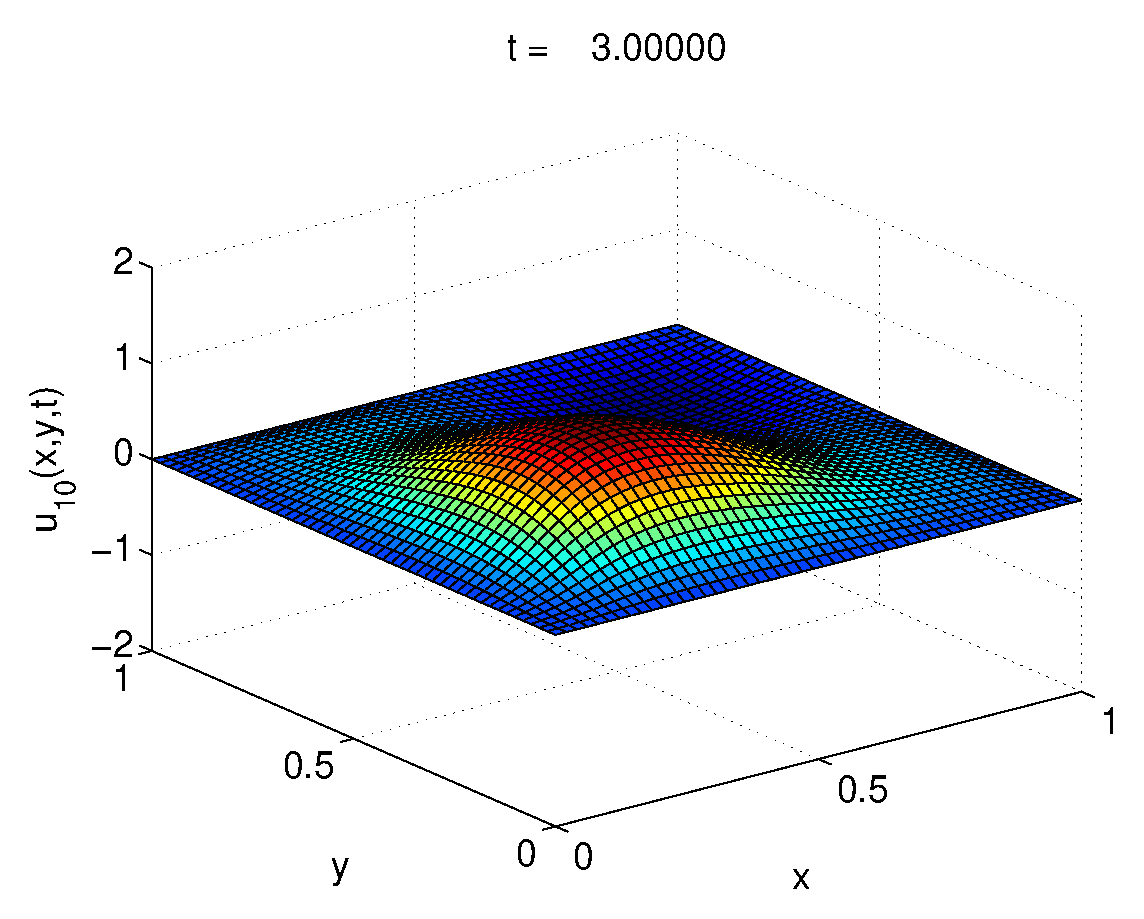
\includegraphics[scale=0.37]{wave2d_6} 
\end{center}

The code that produced these plots follows.

\lstinputlisting{HW44.m}

\end{enumerate}
\end{solution}